% ============================================================
%   CHAPITRE : Probabilités conditionnelles
%   Niveau   : Terminale S
%   Mazava Maths
% ============================================================
\chapter{Probabilités conditionnelles}

\begin{objectifs}
	\begin{itemize}[label=\textbullet]
		\item Calculer une probabilité conditionnelle.
		\item Reconnaître deux événements indépendants.
		\item Utiliser un arbre pondéré pour calculer des probabilités liées à des tirages successifs.
	\end{itemize}
\end{objectifs}


% ============================================================
\section{Probabilité conditionnelle}
% ============================================================

\begin{definition}[Probabilité conditionnelle]
	Soient $A$ et $B$ deux événements avec $\Prob(B) \neq 0$. La \textbf{probabilité de $A$ sachant $B$}, notée $\Prob_B(A)$ ou $\Prob(A/B)$, est définie par :
	\[
	\Prob_B(A) = \frac{\Prob(A\cap B)}{\Prob(B)}.
	\]
\end{definition}

\begin{center}
	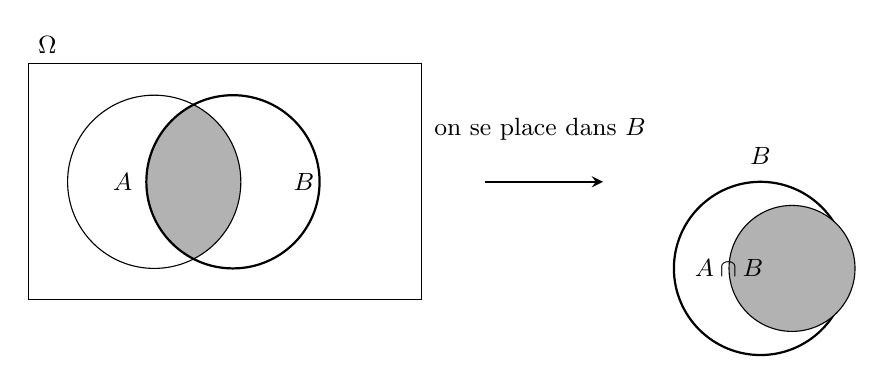
\begin{tikzpicture}[>=stealth, font=\small]
		\draw (0,0) rectangle (5,3);
		\node[above right] at (0,3) {$\Omega$};
		\begin{scope}
			\clip (1.6,1.5) circle (1.1);
			\fill[black!30] (2.6,1.5) circle (1.1);
		\end{scope}
		\draw[thick] (2.6,1.5) circle (1.1);
		\draw (1.6,1.5) circle (1.1);
		\node at (1.2,1.5) {$A$};
		\node at (3.5,1.5) {$B$};
		\draw[->, thick] (5.8,1.5) -- (7.3,1.5);
		\node[above] at (6.5,1.9) {\small on se place dans $B$};
		\begin{scope}[xshift=9.3cm]
			\draw[thick] (0,0.4) circle (1.1);
			\node[above] at (0,1.6) {$B$};
			\fill[black!30] (0.4,0.4) circle (0.8);
			\draw (0.4,0.4) circle (0.8);
			\node at (-0.4,0.4) {$A\cap B$};
		\end{scope}
	\end{tikzpicture}
\end{center}

\begin{astucebac}
	Calculer $\Prob_B(A)$, c'est calculer la probabilité de $A$ en considérant que $B$ devient le nouvel univers de référence.
\end{astucebac}

\begin{exemple}
	Dans une classe, $60\,\%$ des élèves pratiquent un sport ($S$) et, parmi eux, $30\,\%$ pratiquent aussi la musique ($M$). Alors $\Prob(S) = 0,6$ et $\Prob_S(M) = 0,3$, d'où $\Prob(S\cap M) = \Prob(S)\times \Prob_S(M) = 0,18$.
\end{exemple}


% ============================================================
\section{Probabilités composées et arbre pondéré}
% ============================================================

\begin{propriete}{Formule des probabilités composées}{}
	Pour tous événements $A$ et $B$ tels que $\Prob(B)\neq0$ :
	\[
	\Prob(A\cap B) = \Prob(B) \times \Prob_B(A).
	\]
\end{propriete}

Cette formule se lit directement sur un \textbf{arbre pondéré}, dans lequel chaque chemin correspond à une intersection d'événements.

\begin{center}
	\begin{tikzpicture}[>=stealth, grow=right, level distance=2.6cm, sibling distance=4.2cm, font=\small]
		\node (R) at (0,3) {}
		child { node (B1) {$B$} edge from parent node[above] {$\Prob(B)$} }
		child { node (B2) {$\overline{B}$} edge from parent node[below] {$\Prob(\overline{B})$} };
		\begin{scope}
			\path (B1) ++(2.6,1.5) node (A11) {$A$};
			\path (B1) ++(2.6,-1.5) node (A12) {$\overline{A}$};
			\draw[->] (B1) -- (A11) node[above, midway] {$\Prob_B(A)$};
			\draw[->] (B1) -- (A12) node[below, midway] {$\Prob_B(\overline{A})$};
			\path (B2) ++(2.6,1.5) node (A21) {$A$};
			\path (B2) ++(2.6,-1.5) node (A22) {$\overline{A}$};
			\draw[->] (B2) -- (A21) node[above, midway] {$\Prob_{\overline{B}}(A)$};
			\draw[->] (B2) -- (A22) node[below, midway] {$\Prob_{\overline{B}}(\overline{A})$};
		\end{scope}
	\end{tikzpicture}
\end{center}

\begin{methode}
	\textbf{Lire et utiliser un arbre pondéré :}
	\begin{enumerate}
		\item Sur chaque branche issue d'un même nœud, la somme des probabilités vaut $1$.
		\item La probabilité d'un \textbf{chemin} (une suite de branches) est le \textbf{produit} des probabilités inscrites sur ce chemin.
		\item La probabilité d'un événement est la \textbf{somme} des probabilités de tous les chemins qui y conduisent.
	\end{enumerate}
\end{methode}

\begin{propriete}{Probabilités totales (cas de deux issues)}{}
	Si $B$ et $\overline{B}$ forment une partition de $\Omega$ (avec $\Prob(B)\neq0$ et $\Prob(\overline{B})\neq0$), alors pour tout événement $A$ :
	\[
	\Prob(A) = \Prob(B)\times\Prob_B(A) + \Prob(\overline{B})\times\Prob_{\overline{B}}(A).
	\]
\end{propriete}


% ============================================================
\section{Événements indépendants}
% ============================================================

\begin{definition}[Événements indépendants]
	Deux événements $A$ et $B$ sont \textbf{indépendants} lorsque la réalisation de l'un ne modifie pas la probabilité de l'autre, ce qui se traduit par :
	\[
	\Prob(A\cap B) = \Prob(A)\times\Prob(B).
	\]
\end{definition}

\begin{propriete}{Caractérisation}{}
	Si $\Prob(B)\neq0$, les événements $A$ et $B$ sont indépendants si et seulement si :
	\[
	\Prob_B(A) = \Prob(A).
	\]
\end{propriete}

\begin{attention}
	Ne pas confondre \textbf{événements indépendants} ($\Prob(A\cap B)=\Prob(A)\Prob(B)$) et \textbf{événements incompatibles} ($A\cap B=\emptyset$). Deux événements incompatibles de probabilités non nulles ne sont \textbf{jamais} indépendants.
\end{attention}


% ============================================================
\section{Tirages successifs}
% ============================================================

Une urne contient $3$ boules rouges et $2$ boules bleues, indiscernables au toucher. On tire successivement deux boules et on note $R_i$ (resp. $B_i$) l'événement « la $i$-ème boule tirée est rouge (resp. bleue) ».

\subsection{Tirages avec remise}

La boule est remise dans l'urne après le premier tirage : la composition de l'urne ne change pas, les deux tirages sont \textbf{indépendants}.

\begin{center}
	\begin{tikzpicture}[>=stealth, grow=right, level distance=2.6cm, sibling distance=4.2cm, font=\small]
		\node (R) at (0,3) {}
		child { node (B1) {$R_1$} edge from parent node[above] {$\frac35$} }
		child { node (B2) {$B_1$} edge from parent node[below] {$\frac25$} };
		\begin{scope}
			\path (B1) ++(2.8,1.5) node (A11) {$R_2$};
			\path (B1) ++(2.8,-1.5) node (A12) {$B_2$};
			\draw[->] (B1) -- (A11) node[above, midway] {$\frac35$};
			\draw[->] (B1) -- (A12) node[below, midway] {$\frac25$};
			\path (B2) ++(2.8,1.5) node (A21) {$R_2$};
			\path (B2) ++(2.8,-1.5) node (A22) {$B_2$};
			\draw[->] (B2) -- (A21) node[above, midway] {$\frac35$};
			\draw[->] (B2) -- (A22) node[below, midway] {$\frac25$};
		\end{scope}
	\end{tikzpicture}
\end{center}

Les probabilités du second tirage \textbf{ne dépendent pas} du résultat du premier : les branches de niveau $2$ sont identiques.

\subsection{Tirages sans remise}

La boule n'est pas remise : la composition de l'urne change, les tirages sont \textbf{dépendants}.

\begin{center}
	\begin{tikzpicture}[>=stealth, grow=right, level distance=2.6cm, sibling distance=4.2cm, font=\small]
		\node (R) at (0,3) {}
		child { node (B1) {$R_1$} edge from parent node[above] {$\frac35$} }
		child { node (B2) {$B_1$} edge from parent node[below] {$\frac25$} };
		\begin{scope}
			\path (B1) ++(2.8,1.5) node (A11) {$R_2$};
			\path (B1) ++(2.8,-1.5) node (A12) {$B_2$};
			\draw[->] (B1) -- (A11) node[above, midway] {$\frac24$};
			\draw[->] (B1) -- (A12) node[below, midway] {$\frac24$};
			\path (B2) ++(2.8,1.5) node (A21) {$R_2$};
			\path (B2) ++(2.8,-1.5) node (A22) {$B_2$};
			\draw[->] (B2) -- (A21) node[above, midway] {$\frac34$};
			\draw[->] (B2) -- (A22) node[below, midway] {$\frac14$};
		\end{scope}
	\end{tikzpicture}
\end{center}

\begin{exemple}
	Avec remise : $\Prob(R_1\cap R_2) = \dfrac35\times\dfrac35 = \dfrac{9}{25}$.

	Sans remise : $\Prob(R_1\cap R_2) = \dfrac35\times\dfrac24 = \dfrac{3}{10}$.

	On retrouve bien que $\Prob(R_2)$ dépend du résultat du premier tirage dans le second cas : les tirages sans remise ne sont pas indépendants.
\end{exemple}


% ============================================================
\section{Exercices résolus}
% ============================================================

\exerciceresolu
\textbf{Utiliser un arbre pondéré}

Une entreprise fabrique des pièces dans deux ateliers : l'atelier $A$ produit $70\,\%$ des pièces, l'atelier $B$ produit les $30\,\%$ restants. On sait que $2\,\%$ des pièces de l'atelier $A$ sont défectueuses, contre $5\,\%$ pour l'atelier $B$. On prélève une pièce au hasard dans la production totale et on note $D$ l'événement « la pièce est défectueuse ».
\begin{enumerate}
	\item Construire un arbre pondéré représentant la situation.
	\item Calculer $\Prob(A\cap D)$ et $\Prob(B\cap D)$.
	\item En déduire $\Prob(D)$.
\end{enumerate}

\solution

\textbf{1.} On obtient l'arbre suivant, avec $\Prob(A)=0,7$, $\Prob(B)=0,3$, $\Prob_A(D)=0,02$ et $\Prob_B(D)=0,05$ :

\begin{center}
	\begin{tikzpicture}[>=stealth, grow=right, level distance=2.6cm, sibling distance=4.2cm, font=\small]
		\node (R) at (0,3) {}
		child { node (B1) {$A$} edge from parent node[above] {$0,7$} }
		child { node (B2) {$B$} edge from parent node[below] {$0,3$} };
		\begin{scope}
			\path (B1) ++(2.6,1.5) node (A11) {$D$};
			\path (B1) ++(2.6,-1.5) node (A12) {$\overline{D}$};
			\draw[->] (B1) -- (A11) node[above, midway] {$0,02$};
			\draw[->] (B1) -- (A12) node[below, midway] {$0,98$};
			\path (B2) ++(2.6,1.5) node (A21) {$D$};
			\path (B2) ++(2.6,-1.5) node (A22) {$\overline{D}$};
			\draw[->] (B2) -- (A21) node[above, midway] {$0,05$};
			\draw[->] (B2) -- (A22) node[below, midway] {$0,95$};
		\end{scope}
	\end{tikzpicture}
\end{center}

\textbf{2.} $\Prob(A\cap D) = \Prob(A)\times\Prob_A(D) = 0,7\times0,02 = 0,014$.

$\Prob(B\cap D) = \Prob(B)\times\Prob_B(D) = 0,3\times0,05 = 0,015$.

\textbf{3.} $A$ et $B$ formant une partition de l'univers, $D = (A\cap D)\cup(B\cap D)$ avec réunion incompatible, donc :
\[
\Prob(D) = \Prob(A\cap D) + \Prob(B\cap D) = 0,014+0,015 = 0,029.
\]


% ============================================================
\section{Exercices}
% ============================================================

\exercice{Probabilité conditionnelle directe \hfill \facile}

Dans un lycée, $55\,\%$ des élèves sont des filles. Parmi les filles, $40\,\%$ étudient les sciences. On choisit un élève au hasard. Soient $F$ : « l'élève est une fille » et $S$ : « l'élève étudie les sciences ».
\begin{enumerate}
	\item Donner $\Prob(F)$ et $\Prob_F(S)$.
	\item Calculer $\Prob(F\cap S)$.
\end{enumerate}

\exercice{Indépendance \hfill \moyen}

On lance un dé équilibré à six faces. On considère $A$ : « obtenir un nombre pair » et $B$ : « obtenir un multiple de $3$ ».
\begin{enumerate}
	\item Calculer $\Prob(A)$, $\Prob(B)$ et $\Prob(A\cap B)$.
	\item Les événements $A$ et $B$ sont-ils indépendants ? Justifier.
\end{enumerate}

\exercice{Tirages sans remise \hfill \moyen}

Une urne contient $4$ boules vertes et $3$ boules jaunes, indiscernables au toucher. On tire successivement et sans remise deux boules.
\begin{enumerate}
	\item Construire l'arbre pondéré associé à cette expérience.
	\item Calculer la probabilité de tirer deux boules de la même couleur.
	\item Calculer la probabilité de tirer au moins une boule verte.
\end{enumerate}

\exercice{Contrôle de qualité \hfill \difficile}

Une usine produit des composants électroniques à l'aide de deux machines $M_1$ et $M_2$. La machine $M_1$ fournit $65\,\%$ de la production, avec un taux de défaut de $3\,\%$. La machine $M_2$ fournit le reste, avec un taux de défaut de $8\,\%$. On prélève au hasard un composant dans la production totale.
\begin{enumerate}
	\item Représenter la situation par un arbre pondéré.
	\item Calculer la probabilité que le composant provienne de $M_1$ et soit défectueux.
	\item Calculer la probabilité que le composant soit défectueux.
	\item Le composant prélevé est défectueux. Calculer la probabilité qu'il provienne de $M_2$.
\end{enumerate}
